\chapter{Обзор методов обучения с подкреплением и их применения в роботике}\label{ch:ch1}

В настоящее время вычислительные технологии достигли выдающихся результатов. Так обычный процессор спослобен производить до $10^8$ операций в секунду. Однако до недавнего времени компьютер существенно проигрывал человеку в решении сложно формализцемых задач таких как распознавание изображений и анализ текстов на естественном языке. 

Существенный перелом наступил в 2010 году когда с помощью нейронной сети AlexNet было достигнуто качество классификации изображений превосходящее человека. Также в анализе естественного языка был достигнут большой прогресс основанный на применении глубоких нейронных сетей таких как bert. В случае обработки изображений используются наборы данных размеченные человеком. В случае обработки текстов используются не структурированные данные в которых нейронная сеть учится предсказывать следующее слово исходя из контекста. 

Важным подходом для создания общего искусственного интеллекта является обучение с подкреплением \cite{reward_is_enough}. Оно наиболее похоже на то, как обучаются и исследуют мир люди и животные.  


\section{Обзор методов машинного обучения с подкреплением}\label{sec:ch1/sec1}

В современных методах обучения с подкреплением 
Есть много методов
В основном они делятся на два класса 

\subsection{История нейронных сетей}

Перцептрон Розенблата \cite{rosenblatt}
 \cite{Sirotko2, Lukina2, Encyclopedia2, Nasirova2}%
Нейронная сеть как универсальный аппроксиматор
Теорема колмогорова


\subsection{Обучение с подкреплением}

Формализм обучения с подкреплением
Среда, награда, состояние, действия, детерминированные и не детерминированные переходы. Марковский процесс принятия решений МППР, Частично наблюдаемый марковский процесс принятия решений. Задача агента состоит в максимизации суммарной ожидаемой награды в конец эпизода. V-функция, Q-функция

\begin{figure}[ht]
	\centerfloat{
		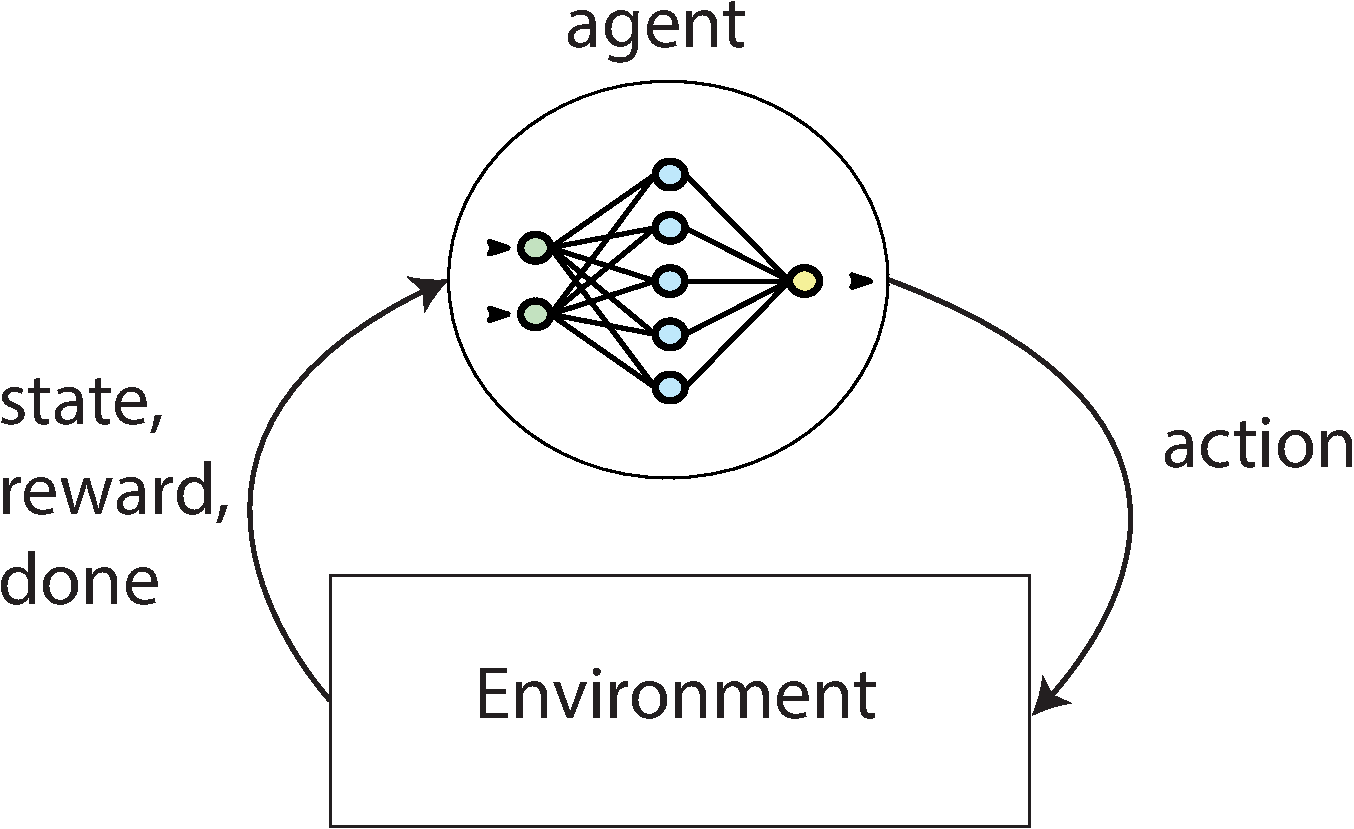
\includegraphics[width=0.5\linewidth]{images/rl_setting}
	}
	\label{img:rl}
	\caption{Взаимодействие агента и среды,}
\end{figure}

\subsection{Уравнение Беллмана}

\begin{equation}
	V^*(s) = \max_{a \in \mathcal{A}} E(r_{t + 1} + \gamma V^*(s_{t + 1}))
\end{equation}

\begin{equation}
Q^*(s, a) = E(r_{t + 1} + \gamma \max_{a' \in \mathcal{A}} Q^*(s_{t + 1}, a'))
\end{equation}
 
\subsection{Value iteration}
Что это
Доказательство сходимости 

\subsection{Policy iteration}
Что это 
Доказательство сходимости

\subsection{Q-learing}
Что это
Пример с табличкой
гамма
метод временных разностей
DQN

\subsection{Policy gradient}
Мотивация 
REINFORCE, Actor-Critic, PPO

\subsection{Meta-learning}
Мотивация MAML, PEARL, RL2

\section{Обзор применения методов обучения с подкреплением в роботике}\label{sec:ch1/sec2}
Перечислить подходы и открытые проблемы (from proposal)


\section{Ссылки}\label{sec:ch1/sec2}


\FloatBarrier
